\section{Data layer}
\label{system-architecture-and-implementation:data-layer}
The benchmark runs on one logical dataset of Norwegian building polygons, materialized in three physical representations: GeoParquet on object storage, server-managed tables in PostGIS, and a Shapefile bundle on local disk. All three derive from the same source data under a single fixed release identifier, \texttt{2026-05-23.1}, so the rows a configuration reads differ only in how they are encoded and stored, never in what they contain. This fixes the dataset across every level, the control established in Section~\ref{research-design-and-methodology:overview-and-experimental-design:factors-and-levels}, so that a difference in transferred bytes or elapsed time traces to the format-and-engine pairing under test rather than to a difference in inputs. A second, fixed dataset of municipality boundaries serves as the join partner in \acrshort{rq}2 and is described at the end of Section~\ref{system-architecture-and-implementation:data-layer:logical-dataset-and-size-tiers}. The subsections below take the logical dataset and its size tiers first, then each physical representation in turn.

\subsection{Logical dataset and size tiers}
\label{system-architecture-and-implementation:data-layer:logical-dataset-and-size-tiers}
The dataset is materialized at three size tiers, small, medium, and large, that realize those defined for the workloads in Section~\ref{research-design-and-methodology:workloads:workload-definitions}. The small tier holds roughly \num{5000000} building polygons and comes directly from the test dataset pipeline, which conflates \acrshort{osm} and \acrshort{fkb} building data into a single deduplicated set. The medium and large tiers are synthesized from it by cloning each source polygon a fixed number of times: the medium tier applies nine clones for a target of roughly \num{40000000} rows, the large tier \num{23} for roughly \num{100000000}. Every clone is translated to a new position within its source county, rotated by a random angle, and perturbed by a small coordinate jitter, and clones whose geometry fails a validity check are discarded. Synthetic clones inherit their source's schema but carry \texttt{NULL} in every non-geometry attribute, so only the originals have populated values. Every row across all three tiers is assigned a \texttt{partition\_key}, a precision-3 geohash\footnote{A geohash encodes a coordinate as a short text string by recursively subdividing the plane into grid cells, so that locations sharing a longer string prefix fall within the same progressively smaller cell.} computed over the polygon centroid in the \acrfull{laea} Europe projection (EPSG:3035), which groups spatially adjacent buildings together for the layout described in the following subsections.

GeoParquet on \acrshort{adls} is the canonical form, written first, and the other two representations derive from it rather than from the source data independently. The test dataset pipeline emits the small tier directly as GeoParquet, and the medium and large tiers are synthesized as GeoParquet from it. The PostGIS tables are then seeded by streaming the GeoParquet rows through DuckDB in chunks, so a full tier is never held in memory during the load, and the Shapefile bundle is exported from the small-tier GeoParquet through DuckDB's \acrshort{gdal} writer. Figure \ref{fig:materialization-lineage} traces this lineage from the canonical GeoParquet form to the derived PostGIS and Shapefile representations. Every representation therefore resolves back to the same GeoParquet rows. The subsections that follow describe each in the order it is produced, beginning with the canonical GeoParquet form.

\begin{figure}[H]
	\centering
	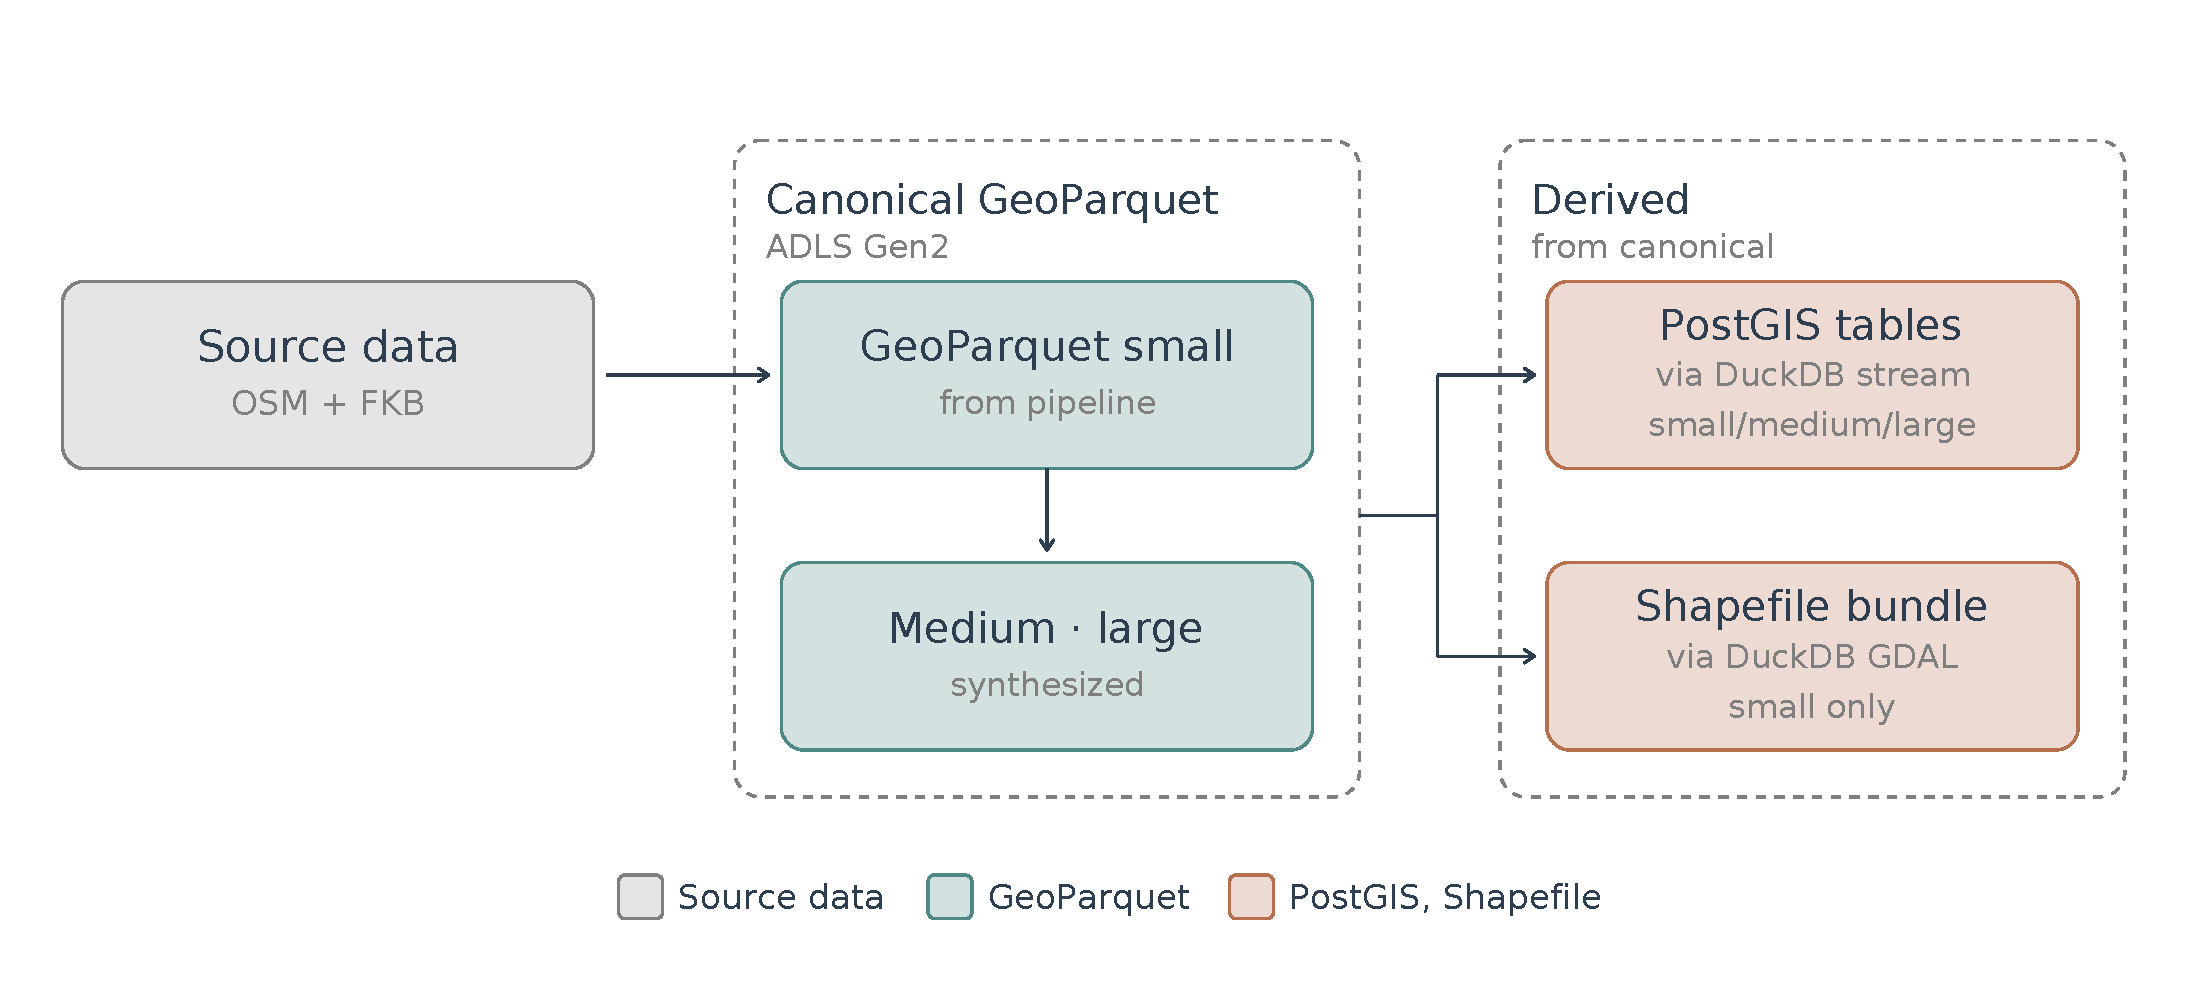
\includegraphics[width=0.8\textwidth]{Chapters/04-system-architecture-and-implementation/sub-chapters/figures/04-materialization-lineage.pdf}
	\caption[Materialization lineage of the three physical representations]{Materialization lineage of the three physical representations. The test dataset pipeline emits the small tier as canonical GeoParquet on \acrshort{adls}, from which the medium and large tiers are synthesized; the PostGIS tables are then derived at all three size tiers by streaming through DuckDB, and the Shapefile bundle is exported from the small tier through DuckDB's \acrshort{gdal} writer.}
	\label{fig:materialization-lineage}
\end{figure}

The benchmark uses a second, much smaller logical dataset of Norwegian municipality boundaries, one polygon per municipality, which serves only the \acrshort{rq}2 spatial join, where each building is associated with the municipality whose boundary contains it (Section~\ref{research-design-and-methodology:workloads:workload-definitions}). Unlike the buildings dataset, this boundary set does not tier: a single fixed collection of roughly \num{360} polygons is reused at every size tier, so only the buildings side of the join grows across small, medium, and large. It is materialized once as a single GeoParquet file, \texttt{municipalities.parquet}, and stored in the \texttt{metadata} container rather than under the per-tier Hive tree\footnote{A Hive-style layout encodes each partition column's value as a \texttt{key=value} segment of the directory path, a convention originating in Apache Hive that lets a reader select partitions by path alone.} of Section~\ref{system-architecture-and-implementation:data-layer:geoparquet-on-adls-gen2}. Sitting outside the buildings materialization lineage of Figure~\ref{fig:materialization-lineage}, it is held constant across every configuration and tier, isolating the buildings dataset as the only input that varies in the join.

\subsection{GeoParquet on ADLS Gen2}
\label{system-architecture-and-implementation:data-layer:geoparquet-on-adls-gen2}

The buildings dataset is written to \acrshort{adls} as GeoParquet conforming to version 1.1.0 of the specification \parencite{ogc2024_geoparquet_specification_v110}. Each partition encodes geometry as \acrshort{wkb}, adds a covering bounding-box column as a struct of \texttt{xmin}, \texttt{ymin}, \texttt{xmax}, and \texttt{ymax}, and is written at a row-group size of \num{100000} rows under snappy compression\footnote{Snappy is a compression codec optimized for speed over compression ratio, so a reader spends little time decoding each row group.}, with its rows sorted by \texttt{partition\_key}. A Hive-style path keyed by release, size, theme, and region organizes the files, taking the form \texttt{\url{release/{release}/size={size}/theme=buildings/region={county}/part\_XXXXX.parquet}}, so one logical release resolves to a tree of per-county GeoParquet files at a fixed size tier.

The layout exposes the dataset to the block-level pruning mechanism described in Section~\ref{background:geometry-and-indexing:spatial-indexing}. The covering bounding box and the per-row-group statistics that Parquet records in the file footer let a reader compare a spatial predicate against each row group's extent and skip those that cannot satisfy it, realizing the range-request access pattern established in Section~\ref{background:spatial-data-formats-and-storage-models:summary}. The region segment of the Hive path extends the same pruning to whole files, so a query bounded to one county reads only the GeoParquet files written under that region rather than the national tree.

\subsection{PostGIS on Azure PostgreSQL}
\label{system-architecture-and-implementation:data-layer:postgis-on-azure-postgresql}

The PostGIS representation materializes the buildings dataset as one table per size tier: \texttt{buildings\_small}, \texttt{buildings\_medium}, and \texttt{buildings\_large}. Each tier resolves to its own table reference at query time, and one server, populated once during setup rather than per benchmark, backs every PostGIS workload across all tiers, so every run reads from a server already in its final state.

PostGIS is installed at run time through the \texttt{azure.extensions} server parameter. Three memory parameters are tuned away from their defaults to suit the analytical workload: \texttt{shared\_buffers} to \SI{2}{\gibi\byte}, \texttt{effective\_cache\_size} to \SI{6}{\gibi\byte}, and \texttt{work\_mem} to \SI{64}{\mebi\byte}. The server \acrshort{sku}\footnote{A SKU, short for stock-keeping unit, is a cloud provider's identifier for one purchasable service configuration, here the managed PostgreSQL instance's compute tier and size.}, region, and compute sizing are fixed in Section~\ref{system-architecture-and-implementation:infrastructure:compute-platforms}. Once a table is loaded, a \acrshort{gist} spatial index named \texttt{\url{buildings\_{size}\_geometry\_idx}} is built on its geometry column, providing the R-tree access method described in Section~\ref{background:spatial-data-formats-and-storage-models:full-database-engines:postgis}, and an \texttt{ANALYZE} refreshes the planner statistics over the freshly loaded rows. Both steps address the stale-statistics threat identified in Section~\ref{research-design-and-methodology:threats-to-validity}, where a planner working from pre-load statistics could misjudge the spatial join.

\subsection{Shapefile bundle}
\label{system-architecture-and-implementation:data-layer:shapefile-bundle}
DuckDB's \acrshort{gdal} writer exports the Shapefile representation from the small-tier GeoParquet, producing the three mandatory components (\texttt{.shp}, \texttt{.shx}, \texttt{.dbf}) alongside a \texttt{.cpg} character-encoding sidecar\footnote{A sidecar file is a small companion file stored beside a primary data file, here carrying the character encoding of the Shapefile's attribute table.}. The coordinate reference system is written separately as a \texttt{.prj} file in the WKT1\_ESRI dialect for EPSG:4326. An OGR\footnote{OGR is the vector-data component of \acrshort{gdal}, the side that reads and writes vector formats such as the Shapefile.} \texttt{CREATE SPATIAL INDEX} call then builds a \texttt{.qix} quadtree index over the bundle, the open-source Shapefile index described in Section~\ref{background:spatial-data-formats-and-storage-models:file-formats:shapefile}. During setup, the completed bundle is uploaded to Blob Storage under the \texttt{copies/shapefile} prefix, and each \texttt{*\_local} entrypoint downloads every component to local disk before its timed window opens, emulating a laptop workflow where the data already sits on the querying machine. The Shapefile is materialized at the small tier only; the GeoPandas entrypoints refuse to run at the medium or large tier, since numbers from those tiers would not be comparable. Reading from local disk leaves the Shapefile with no cloud-native access path, an asymmetry adopted by design and recorded against the comparison it affects in Section~\ref{research-design-and-methodology:threats-to-validity}.